\documentclass[25pt,a1paper,landscape,
               margin=0.5cm,colspace=1.25cm,
               subcolspace=-0.5cm,blockverticalspace=1.25cm]{tikzposter}
\usecolorstyle{Default}
\colorlet{backgroundcolor}{white}

\usepackage[utf8]{inputenc}
\usepackage{amsmath}
\usepackage{amssymb}
\usepackage{listings}
\usepackage{zref-savepos}

\newtheorem{definition}{Definition}
\newtheorem{theorem}{Theorem}

% Remove LaTeX / tikzposter information
\tikzposterlatexaffectionproofoff

% Title based on the example in section 4.1 of the tikzposter documentation
%   P. Richter, E. Botoeva, R. Barnard, and D. Surmann, "The tikzposter class", Jan. 17 2014
\settitle{ \centering \vbox{
    \vspace{1.25cm}
    \centering
    \color{titlefgcolor} {\fontsize{72pt}{72pt}\selectfont \bfseries \sc \@title\\}
    \vspace{1.25cm}
    % Reduce the font size here if necessary to fit all names
    {\fontsize{40pt}{40pt}\selectfont \@author}
    \vspace{1.25cm}
}}

% Defines a block which fills to the bottom of the poster
\newcounter{vfillblockcounter}
\newcommand{\vfillblock}[2]{
    \block{#1}{
        \zsaveposy{vfillblock\the\value{vfillblockcounter}}
        \parbox[t][\zposy{vfillblock\the\value{vfillblockcounter}}sp
                   - \the\TP@blockbodyinnersep - \the\TP@blockverticalspace
                   - \the\paperheight/2 + \the\textheight/2]{\linewidth}{#2}
    }
    \stepcounter{vfillblockcounter}
}

% Some custom colours
\definecolor{custom_grey_0}{rgb}{0.7, 0.7, 0.7}
\definecolor{custom_grey_1}{rgb}{0.2, 0.2, 0.2}
\definecolor{custom_yellow_0}{rgb}{0.99, 0.93, 0.0}
\definecolor{custom_yellow_1}{rgb}{0.98, 0.91, 0.71}
\definecolor{custom_blue}{rgb}{0.54, 0.81, 0.94}

% Poster title
\title{Client Report}
% List of authors
\author{Jue Gong, Xinyi Qian
        \\\hspace*{\fill}\\
        Hymans Robertson LLP}

\begin{document}

% The title
\maketitle[width=0.8\textwidth,roundedcorners=30pt,innersep=0cm,
           titletotopverticalspace=1.25cm,
           titletoblockverticalspace=1.25cm]

% The rest of the poster
\begin{columns}

% First column

\column{0.6}
% First block in the first column
\colorlet{blocktitlefgcolor}{black}
\colorlet{blocktitlebgcolor}{custom_blue}
\colorlet{blockbodyfgcolor}{black}
\colorlet{blockbodybgcolor}{white}
\block{History Performace}{

\begin{figure}[!h]
\centering
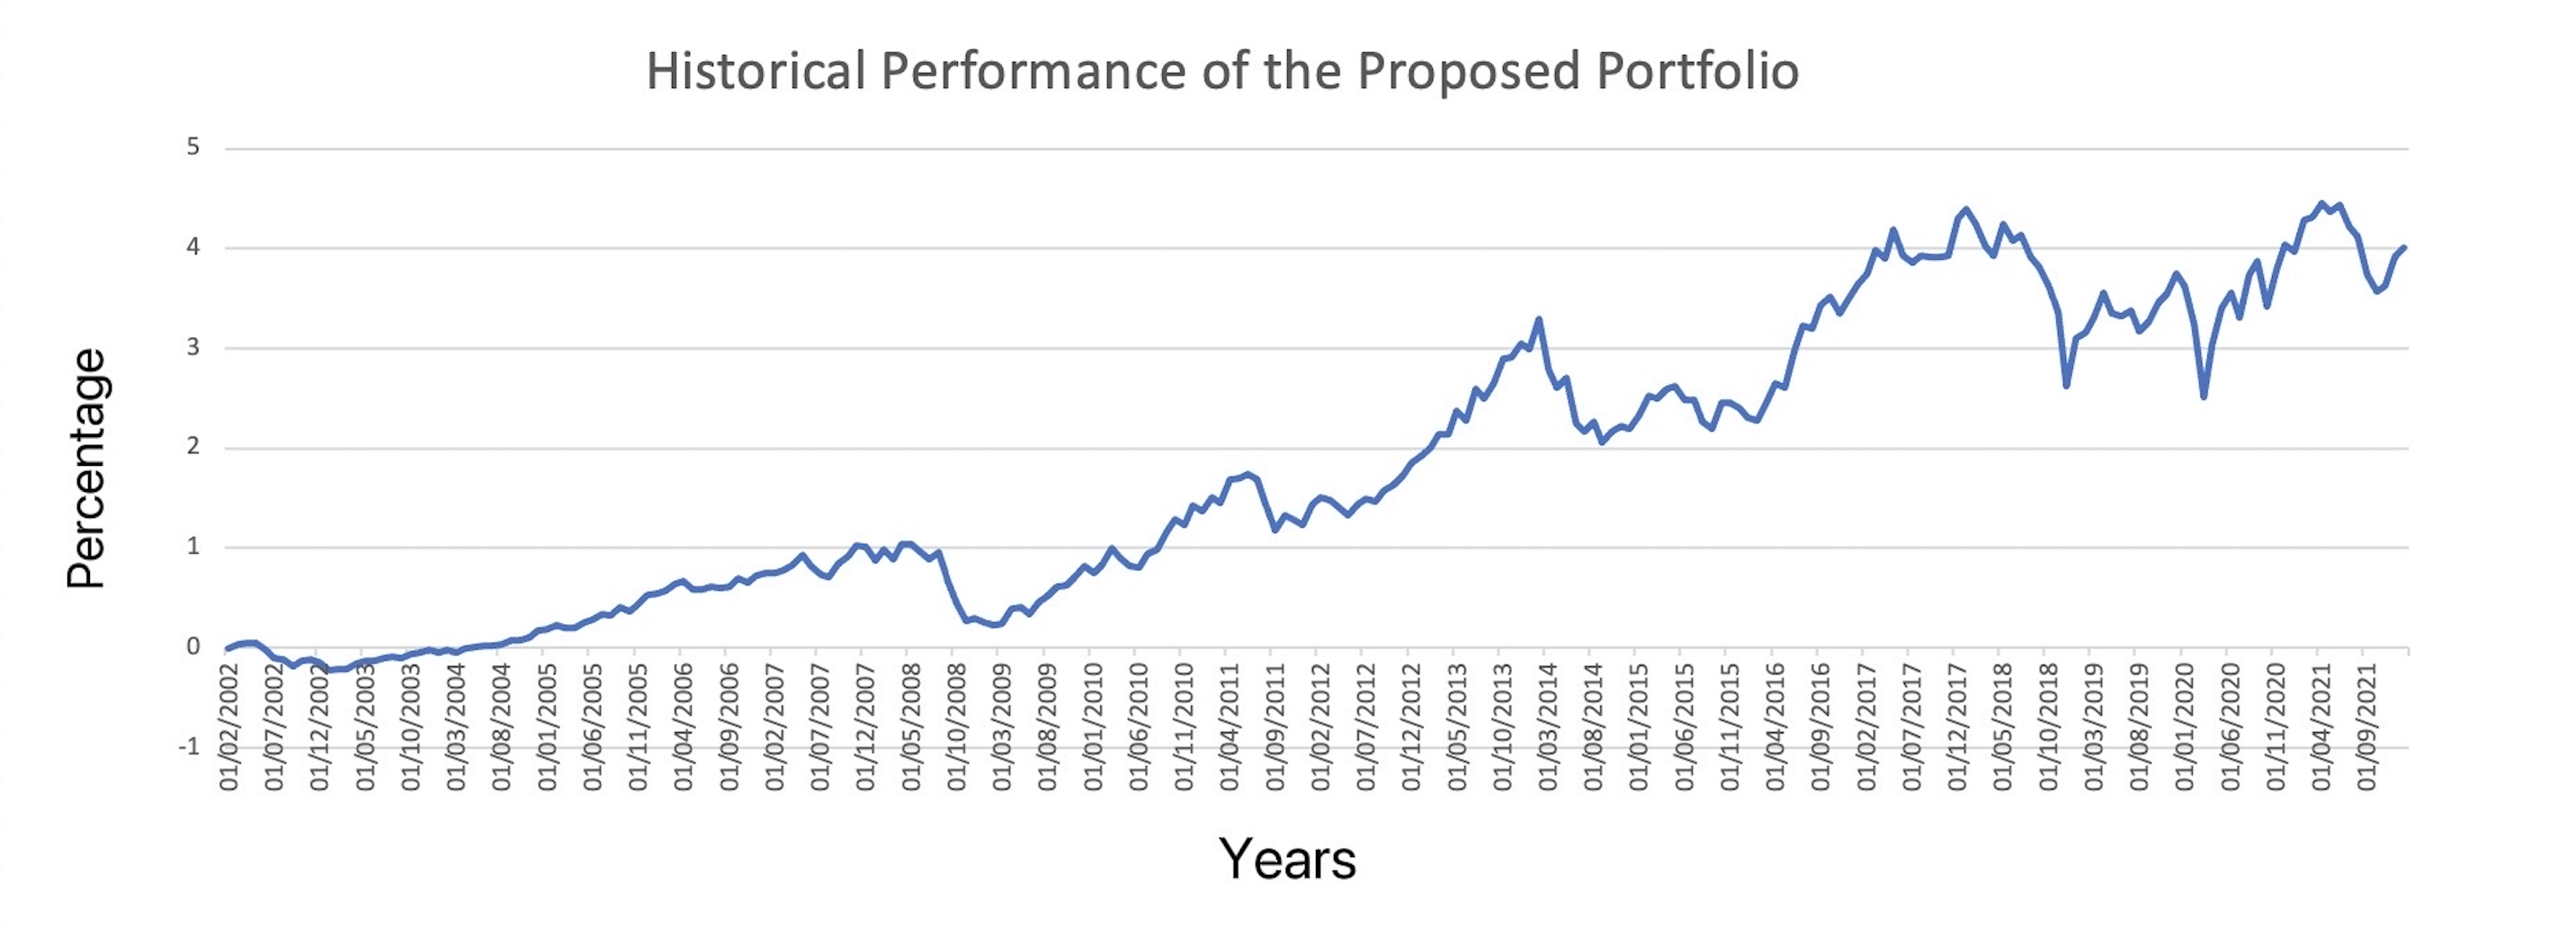
\includegraphics[width=1.0\textwidth]{./Figures/History.png}
\caption{The historical performance of the portfolio.}
\end{figure}

\begin{minipage}[m]{1.0\linewidth}
Our model considers the data of the monthly adjusted closing price of each stock selected in the portfolio for a 20-year period. Over the 20 years period from the January 2002 to the January 2022, the overall prices of the stock combinations increased by approximately 400\%.
\end{minipage}

\begin{center}
\begin{minipage}[m]{1\linewidth}
\begin{tikzfigure}
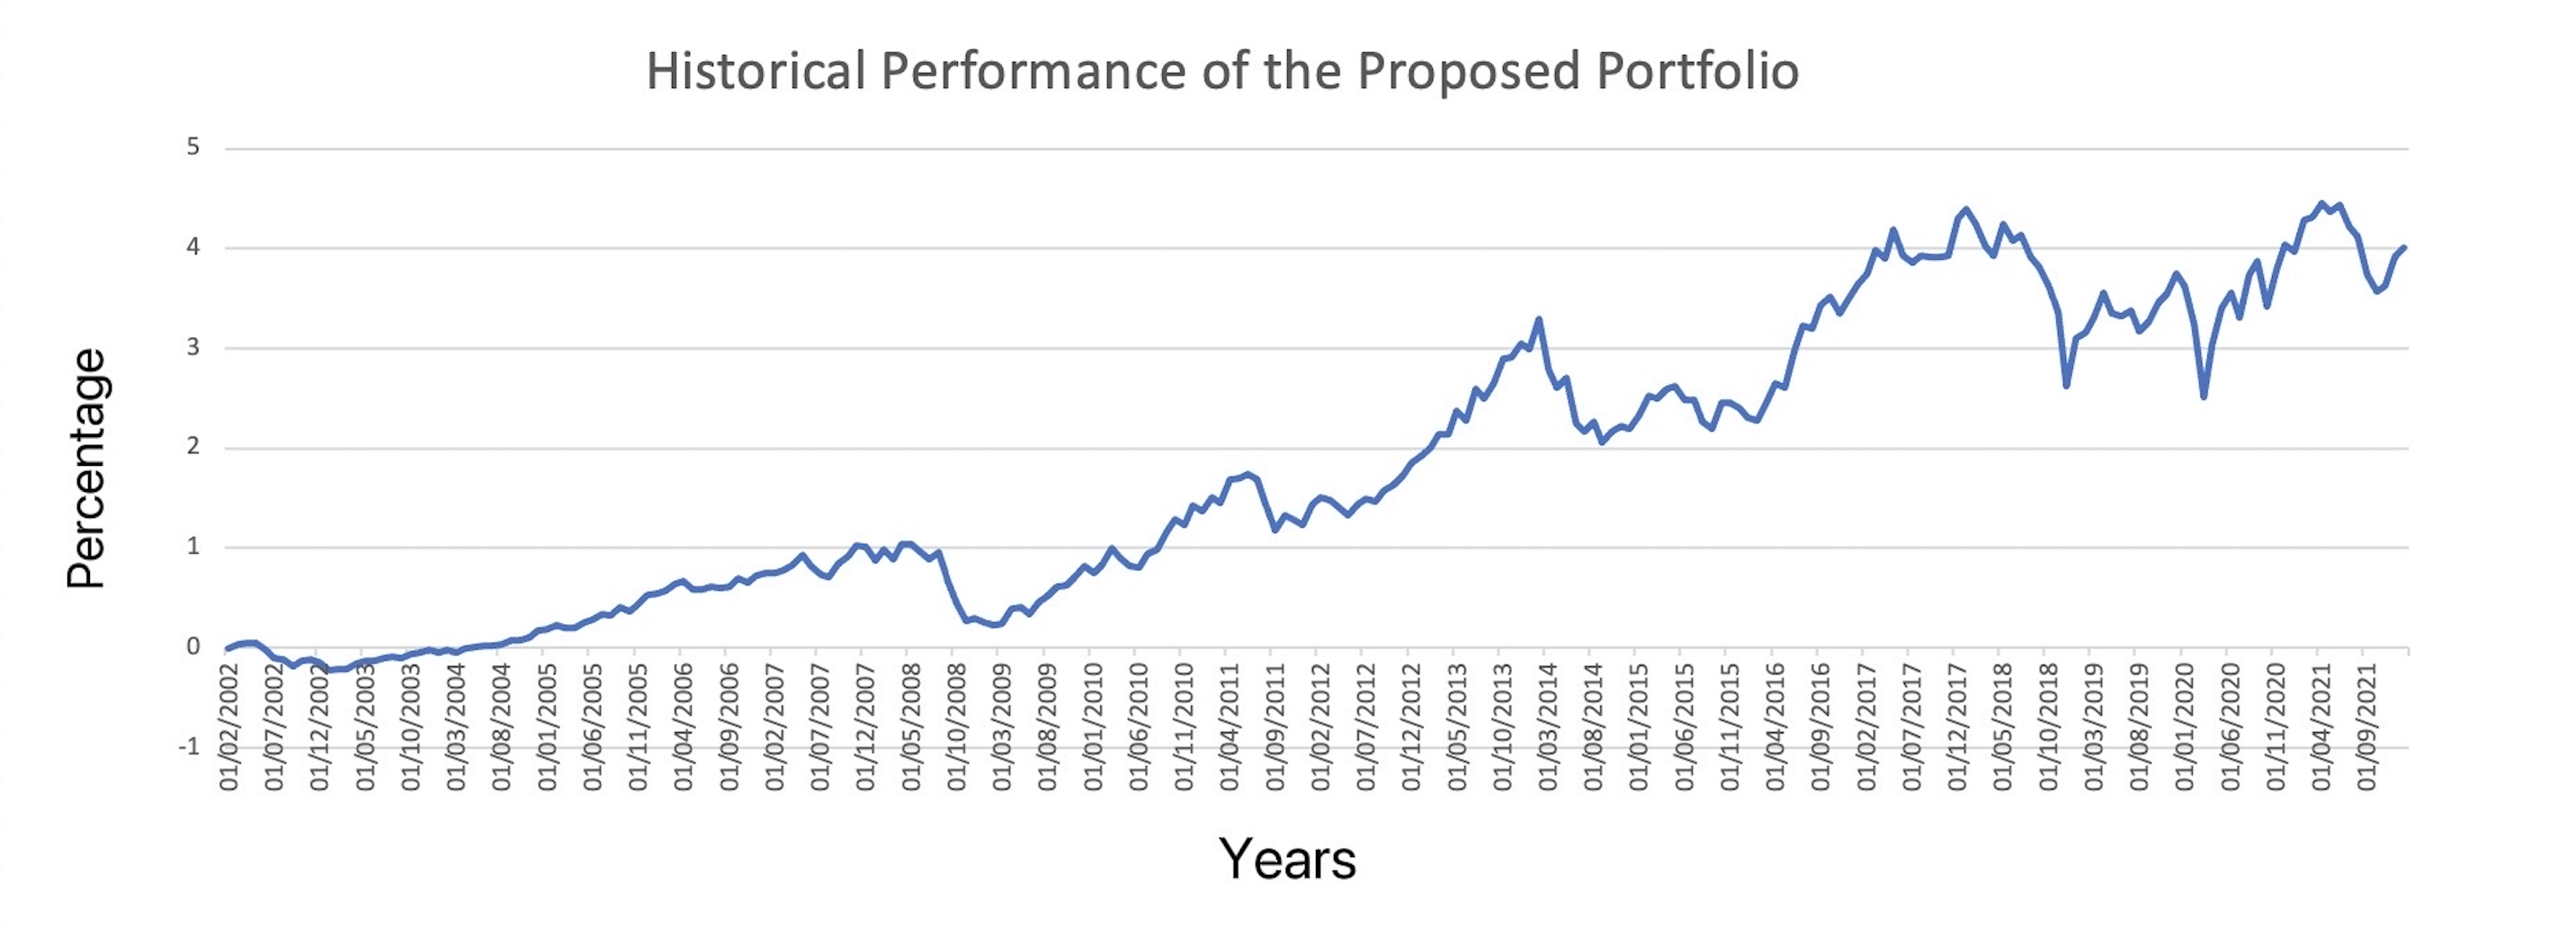
\includegraphics[width=0.6\linewidth]{Figures/History.png}
\end{tikzfigure}
\end{minipage}
\end{center}
}


% Final block in the first column
\vfillblock{Risk Interval and Prospects of the Stock Return}{

\begin{center}
\begin{minipage}[m]{0.9\linewidth}
\begin{tikzfigure}
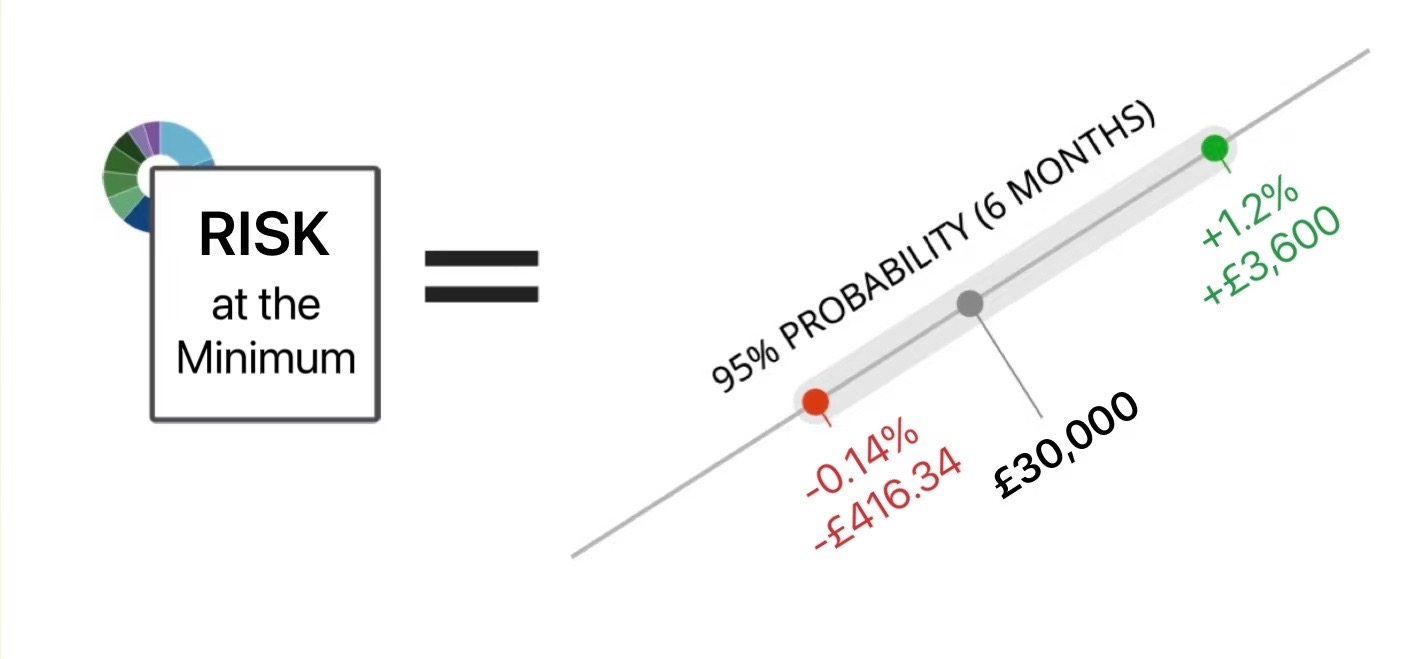
\includegraphics[width=0.8\linewidth]{Figures/Confidence Interval.PNG}
\end{tikzfigure}
\end{minipage}
\end{center}

\begin{minipage}[m]{1.0\linewidth}
Over the next 6-month period, out portfolio is expected to make a stock return of \textit{\pounds}3600, and as little as \textit{\pounds}416.3 for the risk with a 95\% probability.
\end{minipage}
}

% Second column
\column{0.4}
{
\colorlet{blocktitlefgcolor}{black}
\colorlet{blockbodyfgcolor}{black}
\colorlet{blockbodybgcolor}{white}
% First block in the second column
\block{Asset Allocation}{

\begin{center}
\begin{minipage}[m]{1\linewidth}
\begin{tikzfigure}
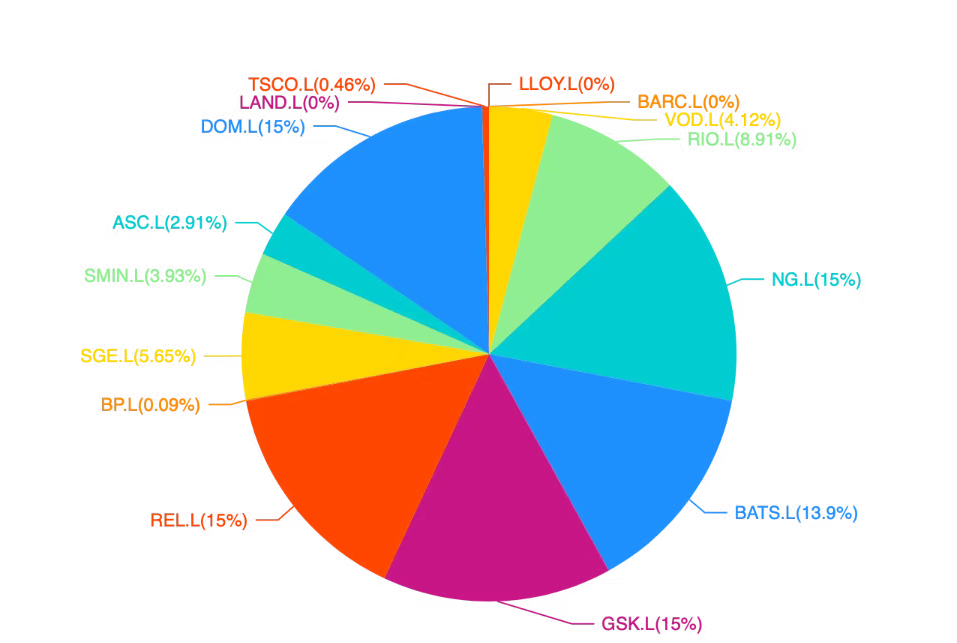
\includegraphics[width=0.7\linewidth]{Figures/optimal.png}
\end{tikzfigure}
\end{minipage}
\end{center}

}
\bigskip
Subcolumns are created using the \texttt{{\textbackslash}subcolumn} command within the \texttt{subcolumns} environment (i.e. between \texttt{{\textbackslash}begin\{subcolumns\}} and \texttt{{\textbackslash}end\{subcolumns\}}). Below, \texttt{{\textbackslash}subcolumn\{0.33\}} creates a subcolumn which spans 33\% of the \emph{column} within which the subcolumns are defined.
}

% Divide the second column into subcolumns
\block{Sector-wise Allocation}{

\begin{center}
\begin{minipage}[m]{1\linewidth}
\begin{tikzfigure}
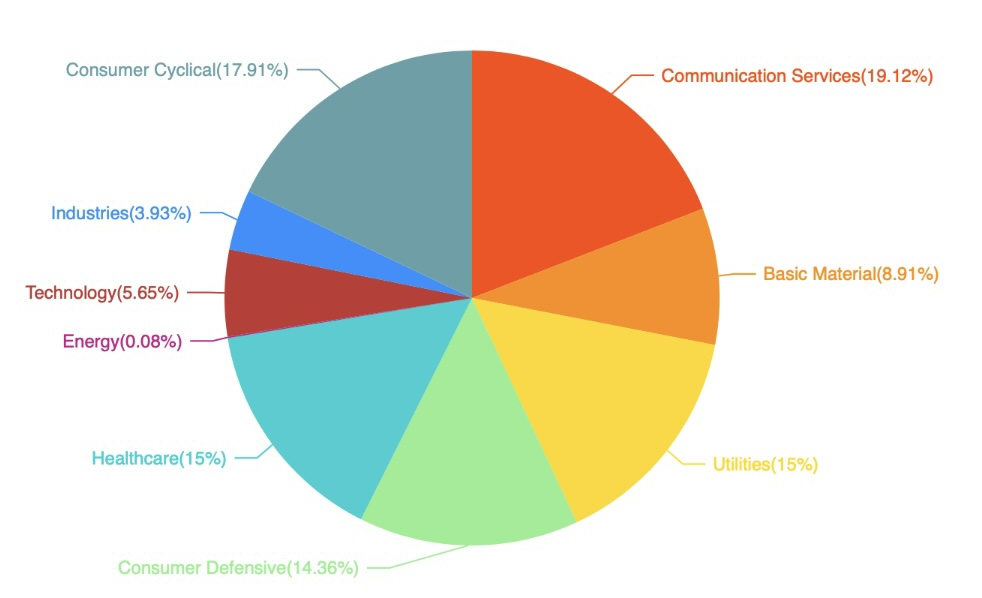
\includegraphics[width=0.7\linewidth]{Figures/Sector-wise Allocation.jpg}
\end{tikzfigure}
\end{minipage}
\end{center}

We suggest our client to invest mainly in 5 sectors: Communication Services, Consumer Defensive, Consumer Cyclical, Utilities and Healthcare. This ensures that the risk is evenly spread out in different sectors that are less correlated to each other.

}

\end{columns}

\end{document}